\chapter{Nondeterminism, Closure Properties, Regular Expressions}

\section{Nondeterminism}

\begin{eg}\label{eg: NFA}
    This is a nondeterministic finite automaton:\\
    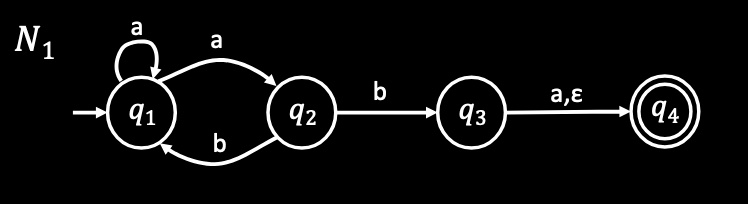
\includegraphics[width=\textwidth]{l2.1.jpg}
    
    What's the difference with what we saw in the last lecture:
    \begin{itemize}
        \item in \(q_1\), when accepting an \(a\), you can either stay in \(q_1\) or go to \(q_2\)
        \item in \(q_1\), if getting \(b\) then there's nowhere to go 
        \item ...
    \end{itemize}

    Example inputs
    \begin{itemize}
        \item \verb|ab| (\textbf{accept} )
        \item \verb|aa| (\textbf{reject} )
    \end{itemize}

\end{eg}

New features of nondeterminism:
\begin{itemize}
    \item multiple paths possible (0, 1 or many at each step)
    \item \(\epsilon\)-transition is a "free" move without reading input
    \item Accept input if \underline{some} path leads to accept state (acceptance overrules rejection) (if one of possible ways to go accepts, then accepts)
\end{itemize}

Nondeterminism doesn't correspond to a physical machine we can build, however it is useful mathematically.

\section{NFA}
\begin{definition}
    A \textbf{nondeterministic finite automaton} is a 5-tuple \(Q, \Sigma, \delta, q_0, F\), where
    \begin{enumerate}
        \item Q is a finite set of states
        \item \(\Sigma\) is a finite alphabet 
        \item \(\delta: Q \times \Sigma_{\epsilon} \Rightarrow \P(Q)\) is the transition function 
        \item \(q_0 \in Q\) is the start state
        \item \(F \subseteq Q\) is the set of accept states   
    \end{enumerate}  

    In which, \(\Sigma_{\epsilon}\) is a shorthand of \(\Sigma \cup \{ \epsilon \} \).  
    P(Q) means the power set of Q which can be represented as \(P(Q) = {R | R \subseteq Q}\), which is the set which contains all the subset of Q.  
\end{definition}

\begin{eg}
    Check the \hyperref[eg: NFA]{NFA example}, we can write transition function such as:
    
    \begin{itemize}
        \item \(\delta(q_1, a) = \{ q_1, q_2 \} \) 
        \item \(\delta(q_1, b) = \emptyset \) 
    \end{itemize}
\end{eg}

Ways to think about nondeterminism: 

Computational view: Fork new parallel thread and accept if any thread leads to an accept state.

Mathematical view: Tree with branches, accept if any branch leads to an accept state.

Magical: Guess at each nondeterministic step which way to go. Machine always makes the right guess that leads to accepting, if possible.

\begin{theorem}
    If an NFA recognizes A then A is regular.
\end{theorem}
\begin{proof}
    By showing how to convert an NFA to an equivalent DFA.
    
    Let NFA \(M = (Q, \Sigma, \delta, q_0, F)\) recognize A, we're going to construct DFA \(M' = (Q', \Sigma, \delta', q'_0, F')\) recognizing A. 

    IDEA: DFA M' keeps track of the \underline{subset of possible states} in NFA M.

    Construct of M':
    \begin{itemize}
        \item \( Q' = P(Q) \)  (States of M' is the power set of Q)
        \item \(\delta'(R, a) = \{ q | q \in \delta(r, a) for \; some \; r \in R\} \) 
        (\(R \in Q'\))
        \item \(q'_0 = \{ q_0 \} \) 
        \item \(F' = \{ R \in Q' | R \; intersects \; F \} \) 
    \end{itemize}
\end{proof}

\begin{remark}
    If M has n states, how many states does M' have by this construction?

    The answer is \(2^n\). 
\end{remark}

Return to \hyperref[theorem: clousre properties union]{Union Closure Property} and \hyperref[theorem: clousre properties concat]{Concatenation Closure Property} by constructing an NFA to prove.

\begin{proof}[Proof: Closure Properties Union]
    N1 corresponds to the DFA M1 recognizes \(A_1\), and N2 corresponds to an input of DFA M2 who recognizes \(A_2\).  

    We can construct an NFA like following:\\
    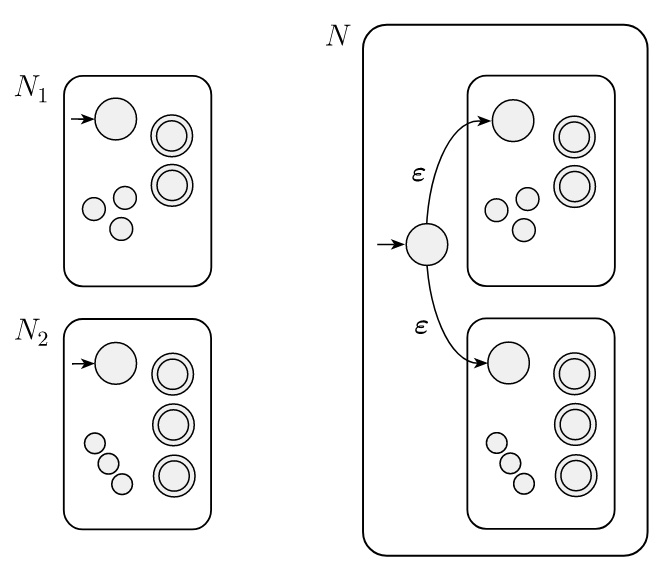
\includegraphics[width=0.8\textwidth]{f1.46.jpg}
\end{proof}

\begin{proof}[Proof: Closure Properties Concat]
     Similar with the last one, this one constructs an NFA recognizes \(A_1A_2\):\\
    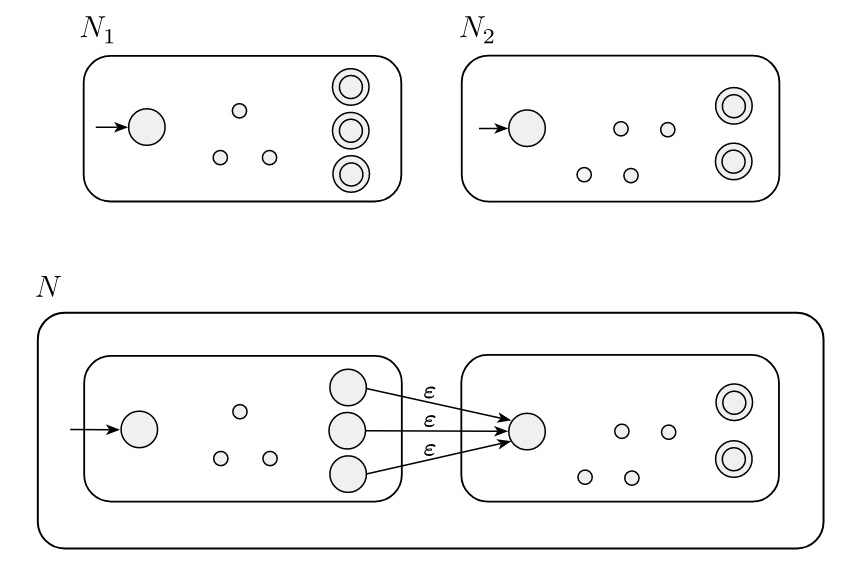
\includegraphics[width=0.8\textwidth]{f1.48.jpg}
\end{proof}

\begin{theorem}[Closure Under Star]
    If A is a regular language, so is \(A*\).  
\end{theorem}
\begin{proof}
    Given DFA \(M\) recognizing A, construct NFA \(M'\) recognizing \(A^*\). 

    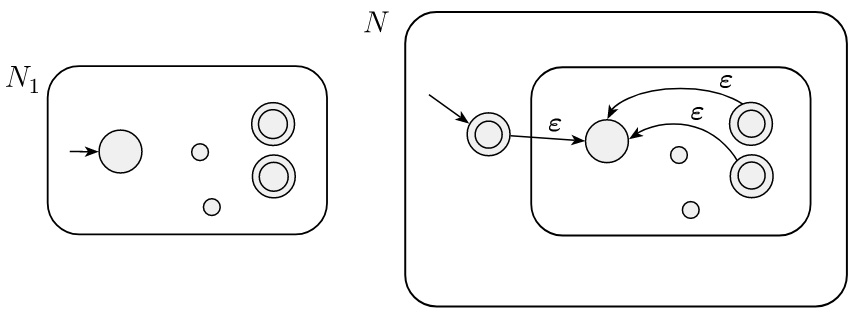
\includegraphics[width=0.8\textwidth]{f1.50.jpg}
\end{proof}
\begin{remark}
    M' have n + 1 states in this construction.
\end{remark}

\begin{theorem}
    If R is regular expression and \(A = L(R)\) then A is regular. 

    That is to say: A language is regular and only if some regular expression describes it.

    This theorem has two directions:
    \begin{lemma}\label{lemma: 2.1}
        If a language is described by a regular expression, then it is regular
    \end{lemma}
    \begin{proof}
        IDEA: Say that we have a regular expression R describing some language A.
        We show how to convert R into an NFA recognizing A.

        When R is \underline{atomic}, we can easily construct NFA for:
        \begin{itemize}
            \item R = a for some \(a \in \Sigma\)
            \item \(R = \epsilon\)
            \item \(R = \emptyset\)   
        \end{itemize}

        When R is \underline{composite}, as we have already constructed for them (closure properties).

        \begin{note}
            This proof works in a recursive way. 
        \end{note}
    \end{proof}

    \begin{lemma}\label{lemma: 2.2}
        If a language is regular, then it is described by a regular expression.  
    \end{lemma}
    \begin{proof}
        This will be proved in next lecture.
    \end{proof}
\end{theorem}
\begin{note}
    Before going to prove this theorem, I need to make some clarifications here.

    \begin{itemize}
        \item \textbf{Regular language}: if some finite automaton recognizes a language, then it is called regular language.
        \item We say a machine recognizes a language if the language is the set contains all the string that can run the machine into an accept state.
    \end{itemize}

    Also we need the definition of \textbf{regular expression} here:
    \begin{definition}
        Say that R is a \textbf{regular expression} if R is
        \begin{enumerate}
            \item \verb|a| for some \verb|a| in the alphabet \(\Sigma\) 
            \item \(\epsilon\)
            \item \(\emptyset\)
            \item \(R_1 \cup R_2\) where \(R_1\) and \(R_2\) are regular expressions
            \item \(R_1 \circ R_2\) where \(R_1\) and \(R_2\) are regular expressions
            \item \(R_1^*\) where \(R_1\) is a regular expression         
        \end{enumerate} 
    \end{definition}
\end{note}


